\section{Описание практической части}
\label{sec:Chapter4} \index{Chapter4}

Для реализации алгоритмов в работе использовался язык программирования Python. Основной причиной в пользу выбора этого языка был тот факт, что тестирующая система DroidBot написана на Python, и для удобного внедрения было принято решение все алгоритмы писать на этом языке. Также Python удобен тем, что предоставляет обширную стандартную библиотеку и множество дополнительных модулей. Это позволяет вести разработку с большой скоростью, без реализации классических алгоритмов.

Реализация большинства подходов ограничивалась стандартной библиотекой  Python. Однако, для некоторых алгоритмов приходилось использовать библиотеки для обработки и визуализации данных: numpy, pandas, matplotlib. Так же для подсчета расстояния редактирования графов была подключена библиотека zss, а для реализации сверточной нейронной сети использовалась библиотека keras.

Все алгоритмы тестирования встраивались в тестирующую систему DroidBot~\cite{li2017droidbot} (Рис.~\ref{InteractionScheme}). Тестирующая система использовалась для того, чтобы основное внимание при решении задачи уделялось реализации алгоритмов тестирования, а не проблемам взаимодействия с устройством. DroidBot состоит из нескольких основных компонентов: \texttt{Device}, \texttt{DeviceState}, \texttt{Environment}, \texttt{InputEvent}, \texttt{InputPolicy}. Все они являются классами языка Python. Класс \texttt{Device} описывает взаимодействия которые происходят с устройством: установка/удаление приложения, получение текущего состояния, получение метаинформации о состоянии, воспроизведение нажатий. Как отмечалось ранее, эти действия происходят через низкоуровневый инструмент Android Debug Bridge. Класс \texttt{DeviceState} отвечает за представление состояния на устройстве, через него также можно получить список интерактивных элементов и возможные взаимодействия с ними. В классе \texttt{Environment} происходит основное взаимодействие тестирующего алгоритма и устройства. В нем задаются настройки тестирования и сохраняются результаты. \texttt{InputEvent} представляет из себя базовый класс для представления произвольного взаимодействия с устройством. Все жесты наследуются от этого класса.

Самым важным для этой работы классом в системе тестирования DroidBot является класс \texttt{InputPolicy}. Это базовый класс всех стратегий тестирования. Для генерации нажатия вызывается метод этого класса \texttt{generate\_event}, который получает на вход обработанное состояние приложения и возвращает действие, которое нужно воспроизвести на устройстве. Это и есть основный цикл, который проходят алгоритмы тестирования.

\begin{figure}[h]
\center{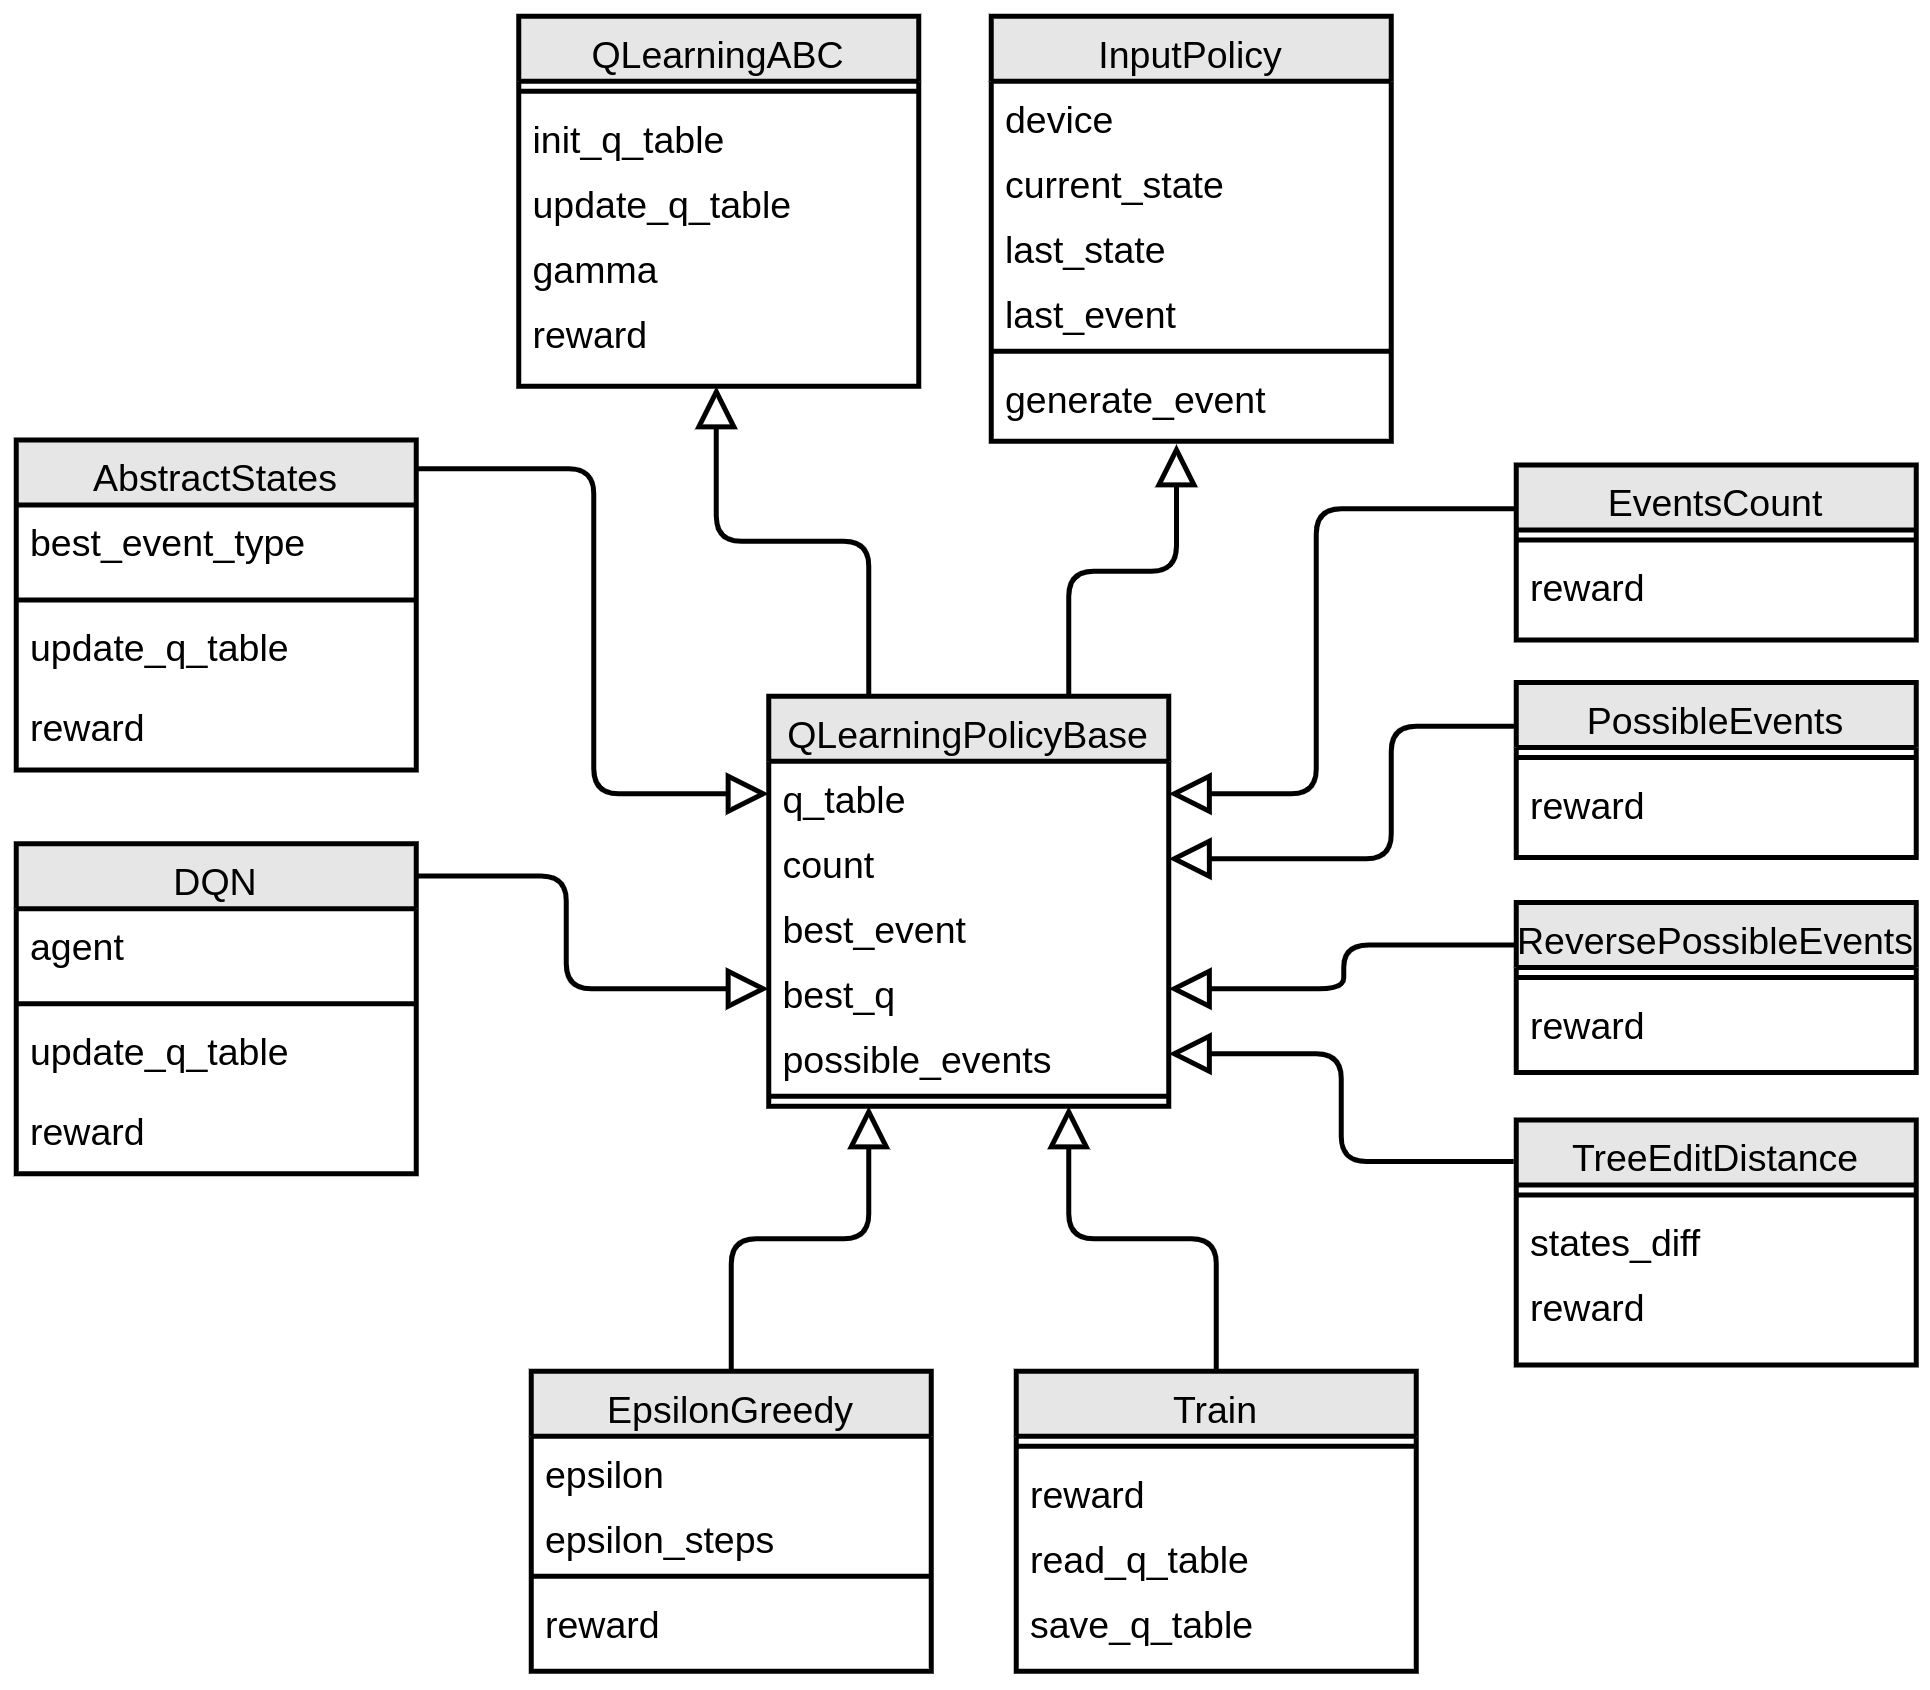
\includegraphics[width=450px]{UMLdiagram.png}}
\caption{UML диаграмма классов стратегий тестирования.}
\label{UML}
\end{figure}

Алгоритмы обучения с подкреплением реализовывались отдельными классами. Их UML диаграмма представлена на Рис.~\ref{UML}. На этой диаграмме можно увидеть два базовых класса: \texttt{QLearningABC} и \texttt{InputPolicy}. Первый содержит абстрактные методы, которые должны быть перегружены в любой Q-learning стратегии, второй -- весь необходимый функционал для встраивания стратегии в DroidBot. Класс \texttt{QLearningPolicyBase} наследует эти два класса и описывает базовую функциональность произвольного Q-learning алгоритма: создание таблицы, подсчет числа взаимодействий, алгоритмы поиска максимального Q-значения и т. д. Все остальные классы на UML диаграмме являются реализацией определенной стратегии из предыдущей главы и наследуются от \texttt{OLearningBase}. 

Все алгоритмы высокоуровнево можно описать одной и той же последовательностью действий:

\begin{enumerate}

\item Ожидание запроса для генерации действия (\texttt{generate\_event})

\item Получение запроса вместе с текущим состоянием (\texttt{generate\_event\_based\_on\_utg})

\item Получение списка возможных взаимодействия в текущем состоянии (\texttt{possible\_events})

\item Поиск лучшего действия согласно Q-таблице (\texttt{update\_best})

\item Обновление Q-значения для предыдущего состояния и действия (\texttt{update\_q\_table})

\item Возврат лучшего действия для воспроизведения на устройстве (\texttt{best\_event})

\end{enumerate}